% QuizForge Backend Documentation - Part 1: Introduction & Architecture
\documentclass[12pt,a4paper]{report}

% Packages
\usepackage[utf8]{inputenc}
\usepackage[T1]{fontenc}
\usepackage{geometry}
\usepackage{graphicx}
\usepackage{tikz}
\usetikzlibrary{shapes.multipart, positioning, arrows.meta, calc}
\usepackage{listings}
\usepackage{xcolor}
\usepackage{hyperref}
\usepackage{tcolorbox}
\usepackage{fancyhdr}
\usepackage{titlesec}
\usepackage{longtable}
\usepackage{array}
\usepackage{booktabs}
\usepackage{enumitem}
\usepackage{pdflscape}

% Page geometry
\geometry{
    a4paper,
    left=25mm,
    right=25mm,
    top=30mm,
    bottom=30mm
}

% Colors
\definecolor{codegreen}{rgb}{0,0.6,0}
\definecolor{codegray}{rgb}{0.5,0.5,0.5}
\definecolor{codepurple}{rgb}{0.58,0,0.82}
\definecolor{backcolour}{rgb}{0.95,0.95,0.92}
\definecolor{javakey}{rgb}{0.5,0,0.35}

% Code listing style
\lstdefinestyle{javastyle}{
    backgroundcolor=\color{backcolour},
    commentstyle=\color{codegreen},
    keywordstyle=\color{javakey}\bfseries,
    numberstyle=\tiny\color{codegray},
    stringstyle=\color{codepurple},
    basicstyle=\ttfamily\footnotesize,
    breakatwhitespace=false,
    breaklines=true,
    captionpos=b,
    keepspaces=true,
    numbers=left,
    numbersep=5pt,
    showspaces=false,
    showstringspaces=false,
    showtabs=false,
    tabsize=2,
    frame=single,
    language=Java
}

\lstset{style=javastyle}

% Hyperref setup
\hypersetup{
    colorlinks=true,
    linkcolor=blue,
    filecolor=magenta,
    urlcolor=cyan,
    pdftitle={QuizForge Backend Documentation - Part 1},
    pdfauthor={System Documentation},
    pdfsubject={Introduction and Architecture},
}

% Headers and footers
\pagestyle{fancy}
\fancyhf{}
\fancyhead[L]{\leftmark}
\fancyhead[R]{QuizForge Backend - Part 1}
\fancyfoot[C]{\thepage}

% Title formatting
\titleformat{\chapter}[display]
{\normalfont\huge\bfseries}{\chaptertitlename\ \thechapter}{20pt}{\Huge}

% Document metadata
\title{%
    \Huge\textbf{QuizForge} \\
    \Large Complete Backend Documentation \\
    \large Part 1: Introduction \& Architecture \\
    \normalsize Version 1.0.0
}
\author{Technical Documentation}
\date{\today}

\begin{document}

% Title page
\maketitle
\tableofcontents
\newpage

% Include chapters for Part 1
% Chapter 1: Introduction
\chapter{Introduction}

\section{Project Overview}

\textbf{QuizForge} is an online quiz platform built with a modern technology stack, providing a comprehensive solution for quiz creation, management, and assessment. The platform supports role-based access control with two distinct user types: Administrators and Candidates.

\subsection{Key Features}

\begin{itemize}[leftmargin=*]
    \item \textbf{Role-Based Access Control (RBAC):} Separate functionalities for ADMIN and CANDIDATE roles
    \item \textbf{Quiz Management:} Create, read, update, and delete quizzes with multiple question types
    \item \textbf{Real-Time Quiz Taking:} Candidates can take quizzes with time tracking
    \item \textbf{Automatic Grading:} System automatically evaluates multiple-choice and true/false questions
    \item \textbf{Analytics Dashboard:} Comprehensive statistics for quiz performance
    \item \textbf{RESTful API:} Complete REST API with OpenAPI 3.0 documentation
    \item \textbf{JWT Authentication:} Secure token-based authentication system
\end{itemize}

\section{Technology Stack}

\subsection{Backend Technologies}

\begin{table}[h]
\centering
\begin{tabular}{|l|l|p{6cm}|}
\hline
\textbf{Technology} & \textbf{Version} & \textbf{Purpose} \\
\hline
Java & 21 & Core programming language \\
\hline
Spring Boot & 3.2.0 & Application framework \\
\hline
Spring Security & 3.2.0 & Authentication and authorization \\
\hline
Spring Data JPA & 3.2.0 & Data persistence layer \\
\hline
PostgreSQL & Latest & Relational database \\
\hline
JWT (JJWT) & 0.11.5 & Token-based authentication \\
\hline
SpringDoc OpenAPI & 2.6.0 & API documentation \\
\hline
Lombok & Latest & Reduce boilerplate code \\
\hline
Bean Validation & 3.2.0 & Input validation \\
\hline
\end{tabular}
\caption{Backend Technology Stack}
\end{table}

\section{Project Structure}

The project follows a standard Spring Boot layered architecture:

\begin{verbatim}
quizforge/
|------ backend/
|   |------ pom.xml                      # Maven configuration
|   \`------ src/main/java/com/quizforge/
|       |------ QuizForgeApplication.java
|       |------ config/                  # Configuration classes
|       |   \`------ OpenApiConfig.java
|       |------ controller/              # REST endpoints
|       |   |------ AuthController.java
|       |   |------ AdminController.java
|       |   \`------ CandidateController.java
|       |------ dto/                     # Data Transfer Objects
|       |------ model/                   # JPA Entities
|       |------ repository/              # Data access layer
|       |------ security/                # Security configuration
|       \`------ service/                 # Business logic
\`------ frontend/                        # React frontend
\end{verbatim}

\section{Design Patterns}

The application implements several industry-standard design patterns:

\begin{enumerate}
    \item \textbf{MVC (Model-View-Controller):} Separation of concerns between data, business logic, and presentation
    \item \textbf{Repository Pattern:} Abstraction layer for data access operations
    \item \textbf{Service Layer Pattern:} Business logic encapsulation
    \item \textbf{DTO Pattern:} Data transfer between layers
    \item \textbf{Builder Pattern:} Used by Lombok for object construction
    \item \textbf{Filter Chain Pattern:} JWT authentication filter
    \item \textbf{Singleton Pattern:} Spring beans are singletons by default
\end{enumerate}

\section{API Architecture}

The API follows RESTful principles with the following characteristics:

\begin{itemize}
    \item \textbf{Resource-Based URLs:} Endpoints represent resources (users, quizzes, attempts)
    \item \textbf{HTTP Methods:} Proper use of GET, POST, PUT, DELETE
    \item \textbf{Stateless:} Each request contains all necessary information
    \item \textbf{JSON Format:} All data exchanged in JSON format
    \item \textbf{HTTP Status Codes:} Meaningful status codes (200, 201, 400, 401, 404, etc.)
    \item \textbf{HATEOAS-Ready:} Structure supports hypermedia links
\end{itemize}

\section{Database Schema Overview}

The application uses six main entities:

\begin{enumerate}
    \item \textbf{User:} Stores user information with role-based access
    \item \textbf{Quiz:} Main quiz entity with metadata
    \item \textbf{Question:} Individual questions belonging to quizzes
    \item \textbf{Option:} Multiple choice options for questions
    \item \textbf{QuizAttempt:} Tracks user quiz attempts
    \item \textbf{Answer:} Stores user responses to questions
\end{enumerate}

\section{Document Organization}

This documentation is organized into the following chapters:

\begin{description}
    \item[Chapter 2: Architecture] Overall system architecture and design decisions
    \item[Chapter 3: Models] Detailed explanation of JPA entities
    \item[Chapter 4: Repositories] Data access layer analysis
    \item[Chapter 5: Services] Business logic implementation
    \item[Chapter 6: Controllers] REST API endpoints
    \item[Chapter 7: Security] Authentication and authorization
    \item[Chapter 8: API Documentation] Complete OpenAPI specification
    \item[Chapter 9: ER Diagram] Database relationships and design
    \item[Chapter 10: Configuration] Application configuration details
    \item[Appendix A: Dependencies] Complete dependency list and versions
\end{description}

\section{Conventions Used in This Document}

\begin{tcolorbox}[title=Code Conventions]
\begin{itemize}
    \item \texttt{Monospace font} indicates code, class names, or file paths
    \item \textbf{Bold text} highlights important concepts
    \item \textit{Italic text} indicates technical terms
    \item Code listings include line numbers for reference
\end{itemize}
\end{tcolorbox}


% Chapter 2: Architecture
\chapter{System Architecture}

\section{Layered Architecture}

QuizForge implements a classic n-tier architecture with clear separation of concerns:

\begin{figure}[h]
\centering
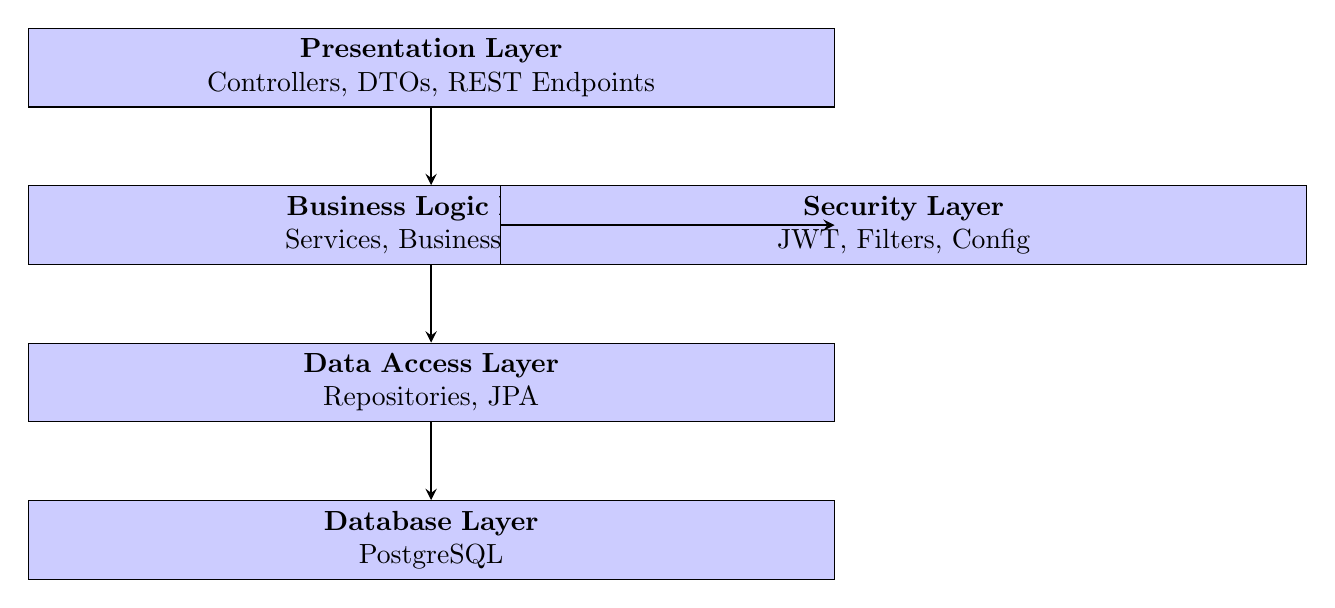
\begin{tikzpicture}[
    layer/.style={rectangle, draw, fill=blue!20, text width=10cm, text centered, minimum height=1cm},
    arrow/.style={->, >=stealth, thick}
]
    \node[layer] (presentation) at (0,0) {\textbf{Presentation Layer} \\ Controllers, DTOs, REST Endpoints};
    \node[layer] (business) at (0,-2) {\textbf{Business Logic Layer} \\ Services, Business Rules};
    \node[layer] (data) at (0,-4) {\textbf{Data Access Layer} \\ Repositories, JPA};
    \node[layer] (database) at (0,-6) {\textbf{Database Layer} \\ PostgreSQL};
    \node[layer] (security) at (6,-2) {\textbf{Security Layer} \\ JWT, Filters, Config};
    
    \draw[arrow] (presentation) -- (business);
    \draw[arrow] (business) -- (data);
    \draw[arrow] (data) -- (database);
    \draw[arrow] (security) -- (business);
\end{tikzpicture}
\caption{System Architecture Layers}
\end{figure}

\subsection{Layer Responsibilities}

\subsubsection{Presentation Layer}
\begin{itemize}
    \item \textbf{Controllers:} Handle HTTP requests and responses
    \item \textbf{DTOs:} Transfer data between client and server
    \item \textbf{Validation:} Input validation using Bean Validation
    \item \textbf{Error Handling:} Exception handling and error responses
\end{itemize}

\subsubsection{Business Logic Layer}
\begin{itemize}
    \item \textbf{Services:} Implement core business logic
    \item \textbf{Transactions:} Manage database transactions
    \item \textbf{Data Transformation:} Convert between entities and DTOs
    \item \textbf{Business Rules:} Enforce application rules and constraints
\end{itemize}

\subsubsection{Data Access Layer}
\begin{itemize}
    \item \textbf{Repositories:} Abstract database operations
    \item \textbf{JPA Entities:} Map to database tables
    \item \textbf{Query Methods:} Define custom queries
    \item \textbf{Relationship Management:} Handle entity associations
\end{itemize}

\subsubsection{Security Layer}
\begin{itemize}
    \item \textbf{JWT Authentication:} Token generation and validation
    \item \textbf{Authorization:} Role-based access control
    \item \textbf{Filters:} Request/response interception
    \item \textbf{CORS:} Cross-origin resource sharing
\end{itemize}

\section{Request Flow}

The typical request flow through the application:

\begin{enumerate}
    \item \textbf{Client Request:} HTTP request arrives at the server
    \item \textbf{JWT Filter:} JwtRequestFilter validates the JWT token
    \item \textbf{Security Context:} Authentication is set in SecurityContext
    \item \textbf{Controller:} Request is routed to appropriate controller method
    \item \textbf{Validation:} Input is validated against constraints
    \item \textbf{Service Layer:} Business logic is executed
    \item \textbf{Repository:} Database operations are performed
    \item \textbf{Response:} DTO is created and returned to client
\end{enumerate}

\begin{figure}[h]
\centering
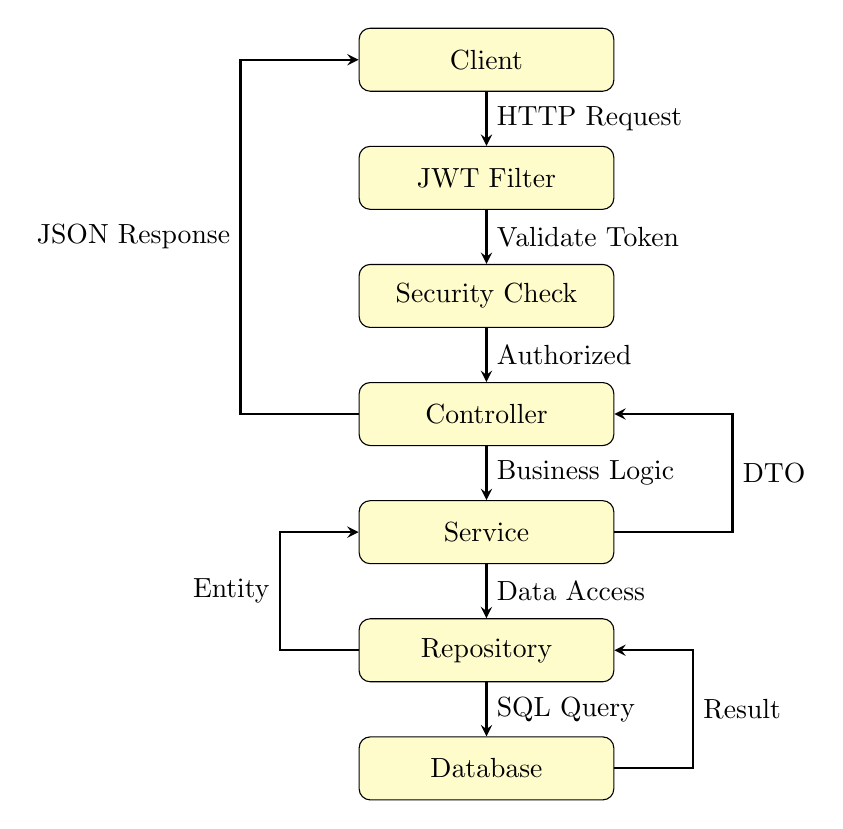
\begin{tikzpicture}[
    node distance=1.5cm,
    box/.style={rectangle, draw, fill=yellow!20, text width=3cm, text centered, minimum height=0.8cm, rounded corners},
    arrow/.style={->, >=stealth, thick}
]
    \node[box] (client) {Client};
    \node[box, below of=client] (filter) {JWT Filter};
    \node[box, below of=filter] (security) {Security Check};
    \node[box, below of=security] (controller) {Controller};
    \node[box, below of=controller] (service) {Service};
    \node[box, below of=service] (repository) {Repository};
    \node[box, below of=repository] (database) {Database};
    
    \draw[arrow] (client) -- node[right] {HTTP Request} (filter);
    \draw[arrow] (filter) -- node[right] {Validate Token} (security);
    \draw[arrow] (security) -- node[right] {Authorized} (controller);
    \draw[arrow] (controller) -- node[right] {Business Logic} (service);
    \draw[arrow] (service) -- node[right] {Data Access} (repository);
    \draw[arrow] (repository) -- node[right] {SQL Query} (database);
    
    \draw[arrow] (database.east) -- ++(1,0) |- node[right, near start] {Result} (repository.east);
    \draw[arrow] (repository.west) -- ++(-1,0) |- node[left, near start] {Entity} (service.west);
    \draw[arrow] (service.east) -- ++(1.5,0) |- node[right, near start] {DTO} (controller.east);
    \draw[arrow] (controller.west) -- ++(-1.5,0) |- node[left, near start] {JSON Response} (client.west);
\end{tikzpicture}
\caption{Request Flow Diagram}
\end{figure}

\section{Component Interaction}

\subsection{Authentication Flow}

\begin{lstlisting}[caption=Authentication Sequence]
1. User sends credentials to /api/auth/login
2. AuthController receives request
3. AuthService validates credentials (simplified for demo)
4. JwtUtil generates JWT token with role
5. LoginResponse with token returned to user
6. User includes token in Authorization header for subsequent requests
7. JwtRequestFilter extracts and validates token
8. SecurityContext populated with authentication
9. Request proceeds to controller with authenticated user
\end{lstlisting}

\subsection{Quiz Creation Flow}

\begin{lstlisting}[caption=Quiz Creation Sequence]
1. Admin sends POST request to /api/admin/quizzes
2. JWT filter validates admin role
3. AdminController receives QuizRequest
4. Bean validation checks input constraints
5. AdminService.createQuiz() called
6. User entity fetched or created
7. Quiz entity created with questions and options
8. CascadeType.ALL persists entire object graph
9. QuizRepository.save() persists to database
10. Entity converted to QuizResponse DTO
11. JSON response returned to client
\end{lstlisting}

\subsection{Quiz Taking Flow}

\begin{lstlisting}[caption=Quiz Taking Sequence]
1. Candidate requests quiz list: GET /api/candidate/quizzes
2. Active quizzes returned without correct answers
3. Candidate starts quiz: POST /api/candidate/quizzes/{id}/start
4. QuizAttempt entity created with IN_PROGRESS status
5. Candidate retrieves questions: GET /api/candidate/quizzes/{id}
6. Questions returned with options (isCorrect hidden)
7. Candidate submits answers: POST /api/candidate/quizzes/submit
8. Answers evaluated against correct options
9. Score calculated and QuizAttempt updated to EVALUATED
10. Results returned to candidate
\end{lstlisting}

\section{Design Decisions}

\subsection{Why Spring Boot 3.2.0?}

\begin{itemize}
    \item Native support for Java 21 features
    \item Enhanced observability and monitoring
    \item Improved startup time and memory efficiency
    \item Built-in support for modern standards
    \item Jakarta EE 10 migration complete
\end{itemize}

\subsection{Why PostgreSQL?}

\begin{itemize}
    \item ACID compliance for data integrity
    \item Advanced indexing capabilities
    \item JSON support for flexible data
    \item Excellent performance with JPA
    \item Wide community support
\end{itemize}

\subsection{Why JWT Authentication?}

\begin{itemize}
    \item Stateless authentication (no server-side sessions)
    \item Scalable across multiple servers
    \item Works well with SPAs and mobile apps
    \item Industry-standard approach
    \item Easy to implement role-based access
\end{itemize}

\subsection{Why Lombok?}

\begin{itemize}
    \item Reduces boilerplate code significantly
    \item Automatic getters, setters, constructors
    \item Builder pattern implementation
    \item Cleaner, more readable code
    \item Compile-time code generation
\end{itemize}

\section{Scalability Considerations}

\subsection{Horizontal Scalability}
\begin{itemize}
    \item Stateless JWT authentication enables load balancing
    \item No session affinity required
    \item Database connection pooling
    \item Can deploy multiple instances behind load balancer
\end{itemize}

\subsection{Database Optimization}
\begin{itemize}
    \item Lazy loading for relationships (LAZY fetch type)
    \item Indexed columns for frequent queries
    \item Batch operations for bulk inserts
    \item Connection pool configuration
\end{itemize}

\subsection{Caching Opportunities}
\begin{itemize}
    \item Quiz data (rarely changes)
    \item User information
    \item Query results for analytics
    \item Second-level cache with Hibernate
\end{itemize}

\section{Error Handling Strategy}

The application handles errors at multiple levels:

\begin{enumerate}
    \item \textbf{Validation Errors:} Bean Validation catches invalid inputs
    \item \textbf{Business Logic Errors:} Services throw RuntimeException with messages
    \item \textbf{Security Errors:} JWT filter returns 401 Unauthorized
    \item \textbf{Database Errors:} JPA handles constraint violations
    \item \textbf{Global Exception Handler:} Can be added for centralized error handling
\end{enumerate}

\section{Transaction Management}

Spring's declarative transaction management is used:

\begin{itemize}
    \item \texttt{@Transactional} annotation on service methods
    \item Automatic rollback on RuntimeException
    \item Propagation defaults to REQUIRED
    \item Isolation level defaults to database default
\end{itemize}



\end{document}
